\begin{block}{Experimental results}
  Experiments been done with two different buffer gas cells.
  \begin{columns}
    \begin{column}{.49\textwidth}
      \begin{center}
      \begin{figure}
        \setlength\fboxsep{0pt}
        \setlength\fboxrule{0.5pt}
        \fbox{\includegraphics[width=.9\linewidth]{figures/1500N2_1500He_buffer}}
      \end{figure}
      1.5 kPa $N_2$ + 1.5 kPa $He$ buffer
      \end{center}
    \end{column}
    \begin{column}{.49\textwidth}
      \begin{center}
      \begin{figure}
        \setlength\fboxsep{0pt}
        \setlength\fboxrule{0.5pt}
        \fbox{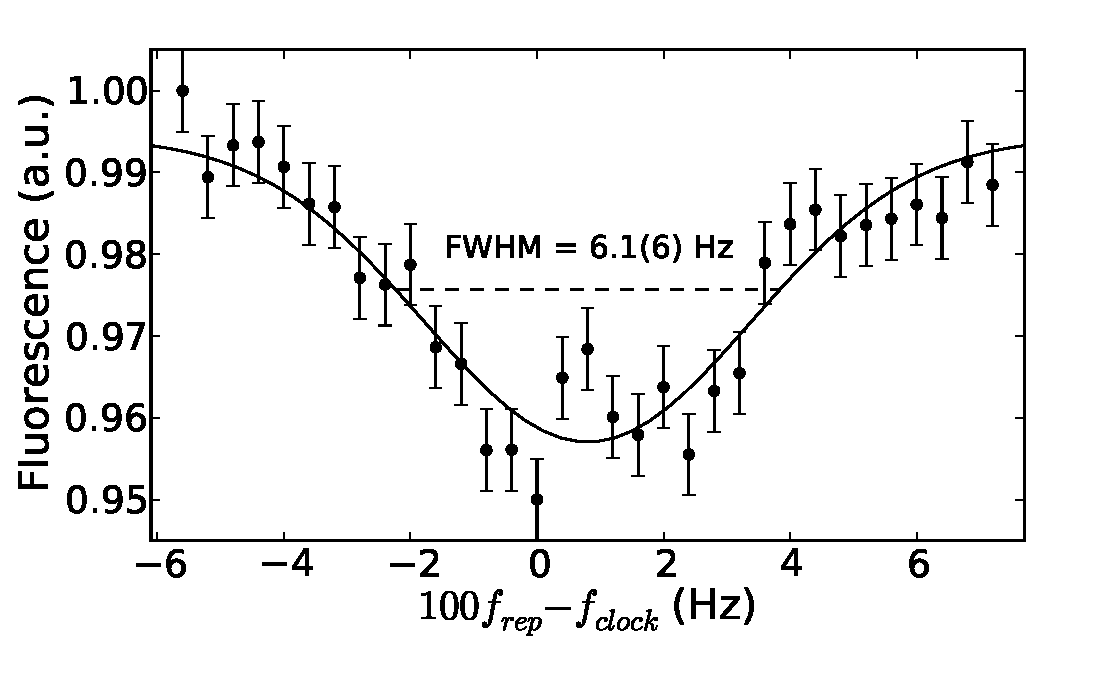
\includegraphics[width=.9\linewidth]{figures/8700Ne_buffer}}
      \end{figure}
      8.7 kPa $Ne$ buffer, $\approx$100$^\circ$C cell wall
      \end{center}
    \end{column}
    \end{columns}
    \begin{itemize}
    \item Higher pressure buffer gas have line-narrowing effect
    \item Pressure and light shift reduced below the uncertainty of the experiment
    \item Signal is sensitive to residual magnetic fields and field inhomogeneities, and temperature change (at $\approx$10$^\circ$C reduced temperature the signal disappears)
    \end{itemize}
\end{block}
